\subsubsection{Speed statics}

In this section, we investigate the average speed and speed distribution for each status. Speed is an important characteristic to define vehicle's behavior.

Fig. \ref{figure_average_speed} shows the average speed when the status is no passenger (status 0) or with passengers (status 1).
 The average speed will increase if there are passengers in taxies. It varies from 25.48 to 27.978 $km/h$ when taxies takes passengers, while it range from 9.977 to 11.272 $km/h$ when taxies are empty. The average speed gap is narrowed when we ignore the records that taxi was motionless. So, we further explore the the proportion taxies stay still in the two status.  Taking the data on March 3, 2011 for example, fig. \ref{figure_speed_is_or_not_0} shows that $64\%$ taxies stopped when there were no passengers in them. But only $23\%$ taxies will stay still when taking passengers.

\begin{table}[!t]
  \centering
  \caption{Average speed statics(km/h)}
\label{table_average_speed}
\vspace{0.1in}
\begin{tabular}{|c|l|l|l|l|l|}
\hline
  Date &$with passengers$&	$no passenger$&	$with passengers,speed!=0$&$no passenger, speed!=0$ \\
  \hline
$2011/3/3 $&	26.57811007&	11.27185805&	34.37218184	& 31.38637735\\
  \hline
$2011/3/4 $&	25.48001368  & 11.27225991& 33.29280414	& 31.25631453\\
  \hline
$2011/3/5 $&	25.55327641	& 10.20210656	& 33.48821719	& 31.29858579\\
  \hline
$2011/3/6 $& 27.97816267	& 9.977911921	 & 35.71509266&32.01122715\\
  \hline
$2011/3/7 $& 27.22384874	& 11.08778299	& 35.00493232	& 31.41230238\\
  \hline
\end{tabular}
\end{table}

\begin{figure}
\centering
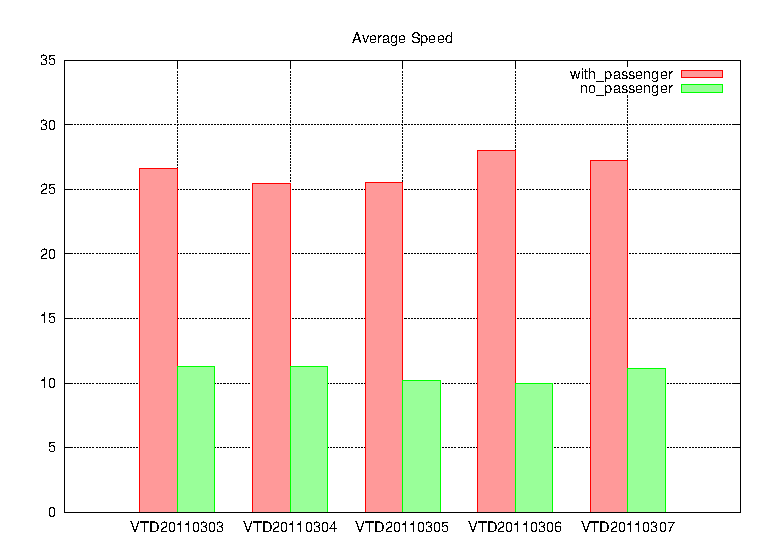
\includegraphics[width=3in]{figures_201103/AverageSpeed.eps}\\
\caption{Average Speed from March 3,2011 to March 7,2011.}\label{figure_average_speed}
\end{figure}


\begin{figure}
\centering
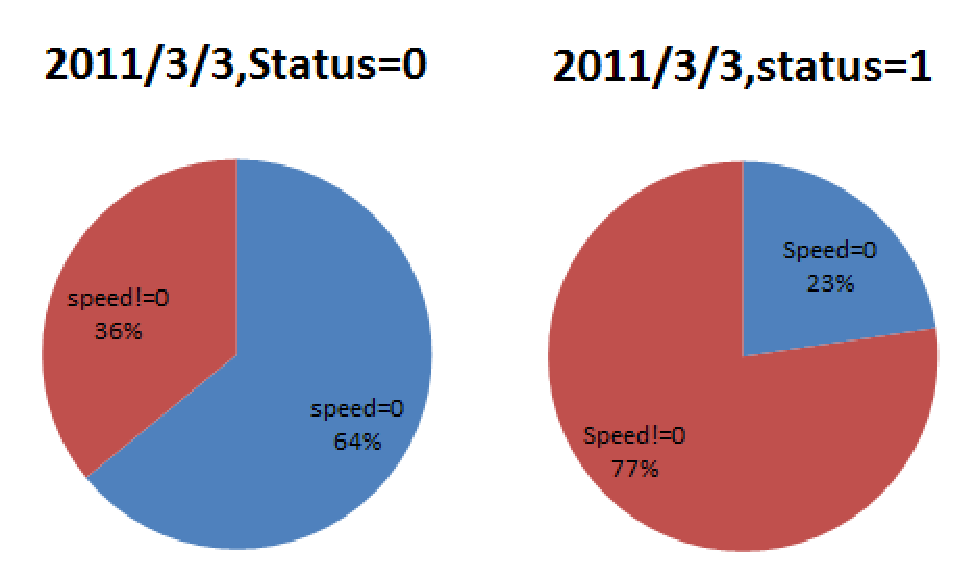
\includegraphics[width=3in]{figures_201103/speed_is_or_not_0.eps}\\
\caption{The proportion of taxies whether speed equals 0.}\label{figure_speed_is_or_not_0}
\end{figure}

Based on \emph{Assumption 1}, we investigate the speed distribution.
%%������μ���ó��ġ�
We calculate the proportion for every speed section, for example, dot(19,0.0245) means $2.45\%$ records fall in the speed range $[19,20)km/h$. Because the proportion for 0km/h reaching up to 20\% is too large compared with the proportion of other speed section, we do not show it in figures.
Fig. \ref{figure_speed_distribution}  show that speed distribution differs for status 0 and 1
 Most speed records are in the speed section $[0,100] km/h$. For status 0, in the speed section (0,40], it follows a linear distribution. But for status 1, there occurs a peak in the $[8,15] km/h$.  Fig. \ref{figure_all_speed_distribution} demonstrates that the speed distribution is with strong regularity for each status.

 The static results are consistent with the \emph{Assumption 1}, that is, the regularity of taxi behavior is similar in each status while it differs between the status.

\begin{figure}[!t]
\centering
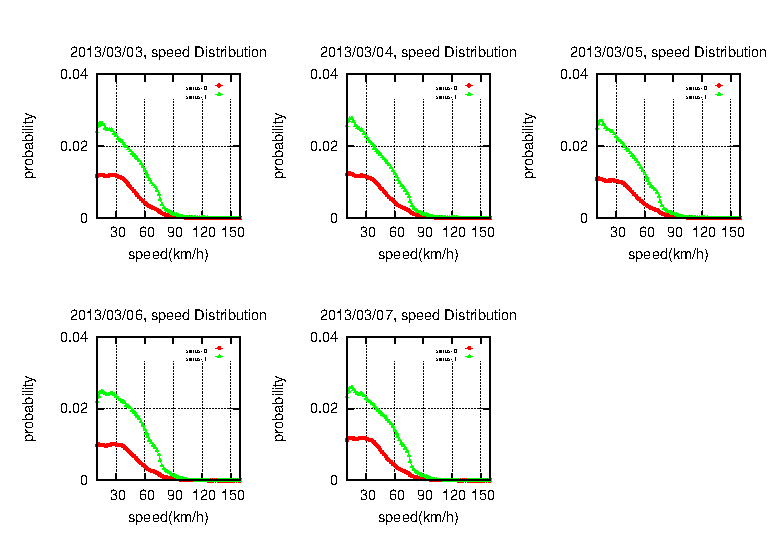
\includegraphics[width=5in]{figures_201103/Speed_distribution.eps}\\
\caption{Speed Distribution for status 0 and 1.Here, red line presents the speed distribution for status 0, and the green one is for status 1. A dot of the line means the proportion of the speed. For example, dot(19,0.0245) means $2.45\%$ records fall in the range $[19,20)km/h$.}\label{figure_speed_distribution}
\end{figure}

\begin{figure}[!t]
\centering
\includegraphics[width=5in]{figures_201103/All_Speed_distribution.eps}\\
\caption{All Speed Distribution for status 0 and 1.}\label{figure_all_speed_distribution}
\end{figure}


